\documentclass[fleqn,10pt]{style}
\usepackage[english]{babel}
\usepackage{lipsum}

\setlength{\columnsep}{0.55cm} % Distance between the two columns of text
\setlength{\fboxrule}{0.75pt} % Width of the border around the abstract

\definecolor{color1}{RGB}{0,0,90} % Color of the article title and sections
\definecolor{color2}{RGB}{0,20,20} % Color of the boxes behind the abstract and headings

\usepackage[superscript,biblabel]{cite}
\usepackage[parfill]{parskip}
\usepackage{booktabs}
\usepackage[justification=centering]{caption}
\usepackage{xcolor}
\usepackage{bm}
\usepackage{multirow}

%	HYPERLINKS
\usepackage{hyperref} % Required for hyperlinks
\hypersetup{
  colorlinks=true,
  breaklinks=true,
  urlcolor=blue,
  citecolor=color1,
  linkcolor=color1,
  bookmarksopen=false,
  pdftitle={Title},
  pdfauthor={Author}
}

% CODE
\usepackage{listings}

\definecolor{White}{rgb}{255,255,255}
\definecolor{Gray}{rgb}{169,169,169}
\definecolor{Blue}{rgb}{0,0,255}
\definecolor{Purple}{rgb}{148,0,211}
\definecolor{DarkGreen}{rgb}{0.0,0.4,0.0} % Comment color
\definecolor{highlight}{RGB}{255,251,204} % Code highlight color

\lstdefinestyle{pythonstyle}{
language=Python,
backgroundcolor=\color{White},
basicstyle=\footnotesize\ttfamily,
breakatwhitespace=false,
breaklines=true,
captionpos=t,
commentstyle=\usefont{T1}{pcr}{m}{sl}\color{DarkGreen},
deletekeywords={},
escapeinside={\%}, % This allows you to escape to LaTeX using the character in the bracket
firstnumber=1,
frame=single, % Frame around the code box, value can be: none, leftline, topline, bottomline, lines, single, shadowbox
frameround=tttt, % Rounds the corners of the frame for the top left, top right, bottom left and bottom right positions
keywordstyle=\color{Blue}\bf, % Functions are bold and blue
morekeywords={}, % Add any functions not included by default here separated by commas
numbers=left, % Location of line numbers, can take the values of: none, left, right
numbersep=10pt, % Distance of line numbers from the code box
numberstyle=\tiny\color{Gray}, % Style used for line numbers
rulecolor=\color{black}, % Frame border color
showstringspaces=false, % Don't put marks in string spaces
showtabs=false, % Display tabs in the code as lines
stepnumber=1, % The step distance between line numbers, i.e. how often will lines be numbered
stringstyle=\color{Purple}, % Strings are purple
tabsize=2, % Number of spaces per tab in the code
}

% Create a command to cleanly insert a snippet with the style above anywhere in the document
\newcommand{\insertcode}[3]{\begin{itemize}\item[]\lstinputlisting[caption=#2,label=#3,style=pythonstyle]{#1}\end{itemize}} % The first argument is the script location/filename and the second is a caption for the listing

%	ARTICLE INFORMATION
\PaperTitle{The Racial Voting Power Gap: Analyzing Racially Polarized Voting with the Discrete Voter Model}

\Authors{Hakeem Angulu\textsuperscript{1}} % Authors
\affiliation{\textsuperscript{1}\textit{Departments of Computer Science and Statistics, Harvard University, Cambridge, Massachusetts, United States}} % Author affiliation
\affiliation{hangulu@college.harvard.edu} % Corresponding author

%	ABSTRACT
\Abstract
{


Section 2 of the Voting Rights Act of 1965 (VRA) \cite{vra} prohibits voting practices or procedures that discriminate based on race, color, or membership in a language minority group, and is often cited by plaintiffs seeking to challenge racially-gerrymandered districts in court.

\medskip

In 1986, with Thornburg v. Gingles\cite{thornburg}, the Supreme Court held that in order for a plaintiff to prevail on a section 2 claim, they must show that:

\begin{enumerate}
  \item the racial or language minority group is sufficiently numerous and compact to form a majority in a single-member district
  \item that group is politically cohesive
  \item and the majority votes sufficiently as a bloc to enable it to defeat the minority’s preferred candidate
\end{enumerate}

All three conditions are notoriously hard to show, given the lack of data on how people vote by race.

\medskip

In the 1990s and early 2000s, Professor Gary King’s ecological inference method tackled the second condition: racially polarized voting, or racial political cohesion. His technique became the standard technique for analyzing racial polarization in elections by inferring individual behavior from group-level data. However, for more than $2$ racial groups or candidates, that method hits computational bottlenecks.

\medskip

A new method of solving the ecological inference problem, using a mixture of contemporary statistical computing techniques, is demonstrated here. It can be used for multiple racial groups and candidates, and is shown to work well on randomly-generated mock election data.
}


\begin{document}

\flushbottom % Make all text pages the same height

\maketitle % Print the title and abstract box

\tableofcontents % Print the contents section

\thispagestyle{empty} % Remove page numbering from the first page

%	ARTICLE CONTENTS

\newpage
\section*{Introduction}

\addcontentsline{toc}{section}{Introduction}

The Voting Rights Act of 1965 (VRA)\cite{vra} was the result of decades of activism and advocacy around unencumbered suffrage in the United States. Specifically, this act was meant to “enforce the fifteenth amendment to the constitution,” which was ratified 95 years prior, and came after African Americans in the South protested the tremendous obstacles to voting they encountered, including poll taxes, literacy tests, harassment, intimidation, physical violence, and other systemic and infrastructural facets of the practical application of the right to vote. The United States Department of Justice has cited it as “the single most effective piece of civil rights legislation ever passed by Congress.”\cite{effective}

Section 2 of that act specifically prohibits any jurisdiction in the nation from implementing any “voting qualification or prerequisite to voting or standard, practice, or procedure...which results in a denial or abridgment of the right of any citizen of the United States to vote on account of race or color.” Today an often challenged voting procedure is the drawing of political districts themselves, on the grounds that gerrymandering dilutes the effectiveness of the vote.

However, quantifying the effects of voting standards on racial groups is notoriously difficult, and both Congress and the Supreme Court have attempted to set aside rules to prove that voting standards that sound neutral have racially disparate effects.

In Thornburg v. Gingles (1986)\cite{thornburg}, the Court established that plaintiffs needed to show that:

\begin{enumerate}[noitemsep]
 \item the racial or language minority group is sufficiently numerous and compact to form a majority in a single-member district
 \item that group is politically cohesive
 \item and the majority votes sufficiently as a bloc to enable it to defeat the minority’s preferred candidate
\end{enumerate}

This amounts to two kinds of evidence, now known colloquially as the Gingles Test, needed to successfully prove a violation of the Voting Rights Act:

\begin{enumerate}[noitemsep]
 \item the geographic conditions to draw an effective district
 \item racial polarization that blocks the will of minority voters
\end{enumerate}

The racially polarized voting test requires showing that a marginalized racial group is \textit{politically cohesive}, and that the “majority votes sufficiently as a bloc to enable it to usually defeat the minority’s preferred candidate.” Both of these are uniquely hard to show given the secret ballot; that is, all voter choices in an election are anonymous. Thus, it is impossible to access the ground truth about how racial groups in the majority and minority vote.

However, statistical methods, most notably King’s Ecological Inference (EI)\cite{king1999}, exist to infer that information from publicly available data.

EI was pioneered in the 1990s and 2000s by Harvard Professor Gary King, and it became the standard technique for attempting to analyze racial polarization in elections in service of mounting VRA litigation. As King himself billed EI, it is “the process of learning about discrete individual-level behavior by analyzing data on groups”\cite{king1999}.

From only the aggregate vote counts and race breakdown, EI produces inferred candidate preferences for each racial group. This is important because the courts that litigate VRA cases do not accept data from non-public sources. Often, this means that the only data that plaintiffs have to bring forward are Census data and election results.

One method of solving the Ecological Inference problem is King's own Ecological Inference method which hinges on Binomial-Beta hierarchical models for Bayesian inference. As a point of departure, this paper explores a new way of providing data to the hierarchical model pipeline: by discretizing the whole parameter space of possible vote outcomes. With this discretized space, one can replace the limited Beta class of distributions with a much more flexible description of voter behavior. This new method for solving the Ecological Inference problem, the \textit{discrete voter model} (DVM), was not computationally tractable in the 1990s and early 2000s, but is now, due to advances in algorithm design and computing power.

While gerrymandering is difficult to prove, it is clear that it is one of the most pressing contemporary voting rights problems. The nation’s electorate, and thus the integrity of the democracy, has to constantly contend with confusing and dilutive maps that are drawn by people, parties, and agencies with specific agendas. It is important that the methods for analyzing redistricting are constantly updated and improved with new knowledge and computing power. Additionally, it is critical that activists, potential plaintiffs, and members of various affected communities all have the ability to quickly and intuitively synthesize the work of mathematicians, statisticians, geographers, political scientists, and other key stakeholders towards resolving this longstanding and nearly intractable problem.

%------------------------------------------------

\newpage
\section{Background}

\subsection{Racial Gerrymandering and the Courts}

Gerrymandering is the practice of creating electoral districts that favor the political interests of specific groups of the electorate in some legislative body. Racial gerrymandering has been affirmed by the court as a direct violation of constitutional rights, with the VRA used to further bolster those rights. A racial gerrymander constitutes a "systemic and infrastructural facet of the practical application of the right to vote," and plaintiffs often invoke the VRA to force officials to redistrict.

Racially polarized voting has been central to redistrcting law since the 1982 amendements to section 2 of the Voting Rights Act.\cite{greiner} This means, practically, that in order to win a lawsuit plaintiffs must prove that voters in districts vote along racial lines.

The \textit{Gingles} decision noted that two techniques were "standard in the literature for the analysis of racially polarized voting"\cite{thornburg}: bivariate ecological regression and homogeneous precints.

Dozens of court cases, from the 1980s to now, have relied on either of the above methods for litigating racial gerrymandering cases\cite{greiner}. However, some appellate courts and judges have been hostile to them. In \textit{Lewis v. Alamance County (1996)}\cite{Lewis_Alamance}, the court said that the critical assumption of regression "runs counter to common sense." In \textit{Holder v. Hall (1994)}\cite{Holder_Hall}, said that "bivariate regression analysis...does not directly control for...factors [other than race]."

These citicisms were often ignored by peer and other courts because they did not posit new ways of deciding cases without using regression. Chief Justice Roberts chimed into the debate as well, saying "At trials, assumptions and assertions give way to facts. In voting rights cases, that is typically done through regression analyses of past voting records."\cite{LULAC}

However, the problem has gotten increasingly more complex. Jim Greiner, Professor of Law at Harvard Law School, stated:

\begin{quote}
 According to some scholars, the patterns themselves have shifted in that a certain percentage of white citizens in some jurisdictions [like Chicago] have become willing to vote for minority-preferred candidates. This shift suggests that the days in which "documenting racially polarized voting is generally...just beating the obvious" may be gone. Racial bloc voting, often a hotly contested issue in an "ordinary" redistricting dispute, may now become even more so, and as a result, using the best methodology is more critical.\cite{greiner}
\end{quote}

Greiner's statement is a good introduction to the future of redistricting. He notes not only that the electorate's voting patterns are becoming more complex, but also that to ensure that the courts are equipped with the correct tools to tackle the complexity, the methodologies supplied by and to expert witnesses must be continually improved.

The ecological regression and homogeneous precints methods had several disadvantages. Ecological regression regularly produces impossible estimates of support, like that $-400\%$ of Hispanic voters in a district supported a candidate. The analysis of homogeneous precincts depends on the assumption that white people living in an all-white precinct vote similarly to white people living in a more racially-diverse precinct, which has been shown empirically, and can be thought intuitively, to be false.\cite{greiner} In addition, neither method generalizes well past $2$ racial groups and $2$ candidates in an election.

The dominant racial bifurcation in both legal and lay discourse is that between Black annd white citizens. Thus, much of the litigation of racial gerrymandering and VRA cases, along with the methods used, have focused on these two groups. However, many contemporary cases explore the more complex racial dynamics that exist in our more, and increasingly, diverse electorate.

Take, for example, a recent case that used ecological regression: \textit{League of United Latin American Citizens v. Perry, 126 S. Ct. 2594 (2006)} (LULAC). In this case, Latinx plaintiffs, a mixture of private citizens and representatives of the Mexican American Legal Defense and Educational Fund, argued that Texas' congressional districts were racially gerrymandered to negatively affect Latinx citizens in Texas. With the help of a dubiously-adjusted ecological regression model (to be used for a larger combination of racial groups), the court decided to throw out District 23 within a new plan proposed in 2003, ordering a remedial redistricting.\cite{LULAC} The court also stated that it need not rule that District 25 was a racial gerrymander, given that the remedial changes to District 23 would necessarily affect District 25.

Although not verbally verified by the court, District 25 is widely believed to have been drawn to pack Latinx voters into a district and dilute their voting power, so the redrawing of it and District 23 was a win for that section of the electorate. The change had incredibly practical, and almost immediate, effects. In the year of the remedial redistricting, the affected districts held new primary elections. Henry Bonilla, the Republican representative for the 23rd congressional district, was defeated by Democrat Ciro Rodriguez, a favorite of the Latinx electorate.

Figure \ref{fig:district25} shows the creation of District 25 after the 2003 redistricting in question. Its shape is reminiscent of popular gerrymanders.

\begin{figure*}[ht]\centering
 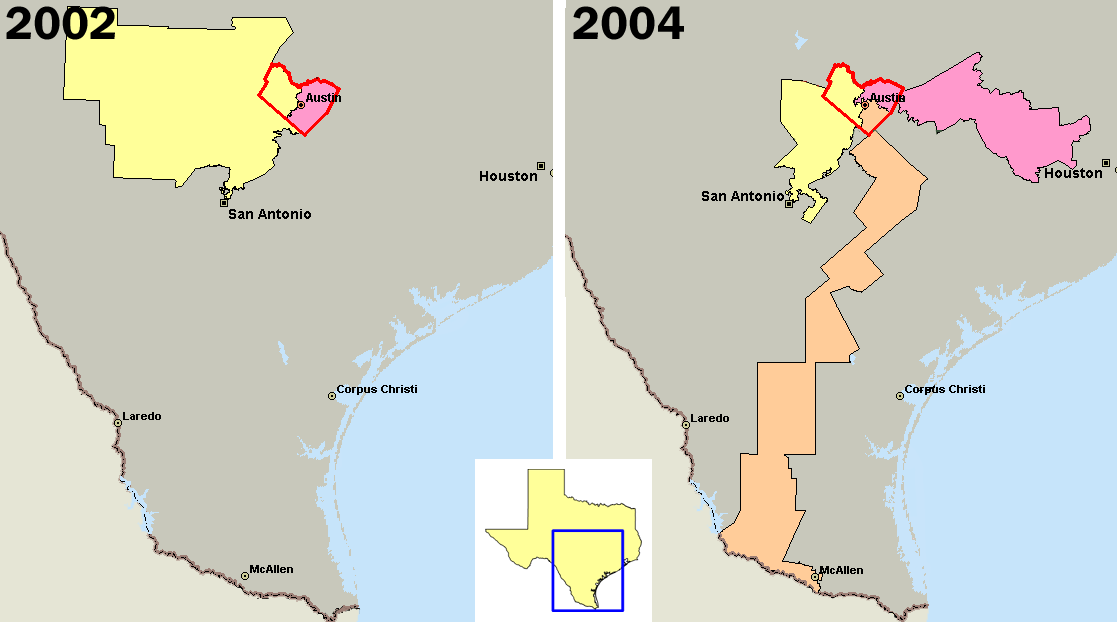
\includegraphics[width=.75\linewidth]{images/district25.png}
 \caption{The Creation of Texas' 25th Congressional District (orange) in 2003\cite{district25}}
 \label{fig:district25}
\end{figure*}

In that decision, the judges referred to a previous one from 1993, where the court stated:

\begin{quote}
 In countless areas of the law weighty legal conclusions frequently rest on methodologies that would make scientists blush. The use of such blunt instruments in examining complex phenomena and corresponding reliance on inference owes not so much to a lack of technical sophistication among judges, although this is often true, but to an awareness that greater certitude frequenetly may be purchased only at the expense of other values.\cite{clements}
\end{quote}

Here, the court explicitly acknowledges the disadvantages of the methods used to infer racially polarized voting. These disadvantages, the criticisms lain on ecological regression and homoegenous precincts by some courts, and improvements in theory inspired a burst of energy and innovation in the academy in the late 1990s and early 2000s. At the center of this burst is King's EI.

\subsection{Ecological Inference}

\textit{Ecological inference} is the process of using aggregate (or, ecological) data to infer discrete individual-level relationships of interests when individual-level data are not available.\cite{king1999} This is distinct from the \textit{ecological regression} discussed above, which is the statistical method of running regressions on aggregates and interpreting those regressions as predictive relations on the level of individual units.\cite{ec_reg}

In a world with two categories, groups $1 \rightarrow \dots$ and groups $A \rightarrow \dots$, both methods seek to answer the question "what percentage of members in group $1$ are also in group $A$?" This is precisely the answer that plaintiffs need in racial gerrymandering cases, where groups $1 \rightarrow$ are races and groups $A \rightarrow$ are candidates.

Greiner provides an alternate description of EI that fits well within mathematical models.\cite{greiner} EI can also be understood as the attempt to predict internal cell values of a set of contingency tables, like Table \ref{table:ei_example}, when only the column and row totals (the margins of the table) are observed.

\begin{table}
 \centering
 \caption{A $3 \times 3$ Table of Voting By Race, using Counts of Voting Age Population}
 \label{table:ei_example}
 \begin{tabular}{cccc}\toprule
         & Cand. 1       & Cand. 2       & $\sum$        \\\midrule
  Race 1 &      -         &       -        & Race 1 Pop.   \\
  Race 2 &     -          &      -         & Race 2 Pop.   \\
  $\sum$ & Cand. 1 Votes & Cand. 2 Votes & Precinct Pop.
 \end{tabular}
\end{table}

Each precinct has its own table, with an election's vote counts as the column totals and the voting age population, or demographic split of the district, often from the Census, as the row totals. The internal cells, how many people of each racial group that voted for each candidate, are protected by the secret ballot. Those internal cells are exactly the evidence needed in racial gerrymandering litigation, and their values have been inferred by ecological regression and homogeneous precinct analysis in the past.

Theoretically, these tables can be expanded to be as large as necessary $\rightarrow R \times C$, where $R$ corresponds to the number of rows (demographic groups or races) and $C$ corresponds to the number of columns (candidates). This would be ideal given that the diversification of the electorate has created more politically powerful demographic groups, and that there are frequently more than $2$ candidates in elections, especially in local cases (where many infringements of the VRA occur).

Professor Gary King developed and proposed his own method to solve this problem in the late 1990s. It has been used in a few court cases, mainly for the advantage that unlike ecological regression, this method will never produce impossible estimates. It is also understood to be more intuitive than regression, addressing the court's seldom complaint.

King's EI uses Bayesian inference and bounds methods to infer the values of the empty cells in Table \ref{table:ei_example}.

Using Table \ref{table:ei_example} as a reference, Table \ref{table:ei_quantities} describes the quantities that King used to describe this problem\cite{king1999}.

\begin{table*}[ht]
 \centering
 \caption{Quantities in King's EI}
 \label{table:ei_quantities}
 \begin{tabular}{|l|l|}
  \hline
  \multicolumn{1}{|c|}{Quantity} & \multicolumn{1}{|c|}{Description}                           \\
  \hline
  \multicolumn{2}{|c|}{Observed}                                                               \\
  \hline
  $X_i$                          & fraction of population $i$ in race $1$                      \\
  $T_i$                          & fraction of population $i$ who voted for candidate $1$.     \\
  $N_i$                          & size of population $i$                                      \\
  $T'_i$                         & number of people in population $i$ in race $1$              \\
  \hline
  \multicolumn{2}{|c|}{Unobserved}                                                             \\
  \hline
  $b1_i$                         & fraction of members of race $1$ who voted for candidate $A$ \\
  $b2_i$                         & fraction of members of race $2$ who voted for candidate $A$ \\
  \hline
 \end{tabular}
\end{table*}

King's method then uses the observed quantities, and a few parameters, to find the unobserved quantities and answer the ecological inference question. The parameters used are described in Table \ref{table:ei_params}.

\begin{table*}[ht]
 \centering
 \caption{Parameters in King's EI}
 \label{table:ei_params}
 \begin{tabular}{|l|l|}
  \hline
  \multicolumn{1}{|c|}{Parameter} & \multicolumn{1}{|c|}{Description}                                     \\
  \hline
  $c_1, d_1$                     & hyperparameters for the Beta distribution for $b_1$                   \\
  $c_2, d_2$                     & hyperparameters for the Beta distribution for $b_2$.                  \\
  $\theta$                       & the expected fraction of the population of $i$ registered to vote $i$ \\
  $\lambda$                      & the fixed hyperparameter for the distributions of $c_1, c_2, d_1, d_2$ \\
  \hline
 \end{tabular}
\end{table*}

The model is a hierarchical Bayesian inference model that proceeds as follows:

\begin{enumerate}
 \item $c_1, c_2, d_1, d_2 \sim \text{Exponential}(\lambda)$
 \item $b1_i | c_1, d_1 \sim \text{Beta}(c_1, d_1)$
 \item $b2_i | c_2, d_2 \sim \text{Beta}(c_2, d_2)$
 \item $T'_i | b1_i, b2_i, X_i \sim \text{Binomial}(N_i, \theta_i)$
\end{enumerate}

The Python implementation of King's EI is given in Listing \ref{lst:ei_code}. Using the observed quantities, King's method produces a model for the unobserved quantities of interest, which can then be used in litigation as described above.

However, in King's original paper, the bulk of his examples are for $2 \times 2$ tables, and proposed extensions of that method beyond that bound have been dubious.

In King's second iteration of his method and accompanying software, \textit{EI2}, King implements a "Multiple Imputation Approach" to try to handle $2 \times 3$ tables. In essence, this approach collapses the $2 \times 3$ table into multiple $2 \times 2$ subtables, then applies the original method to each of those subtables.\cite{king2013} Statisticians and scholars, like Jim Greiner, have noted that this method as applied is statistically invalid, as it does not, and cannot, fully adhere to combinatorial rules that the pioneer of multiple imputation, Professor Donald Rubin of Harvard University, notes in his writings.\cite{rubin}

The problems increase if the size of the table increases to $3 \times 3$ or higher. Professor Karen Farree of the University of California, San Diego investigated King's EI applied to tables of that size, and found that the method produced biased estimates and relied on inappropriate modeling assumptions.\cite{ferree}

With an increasingly diverse electorate, and complex multi-candidate elections, a method that generalizes well to an $R \times C$ table, with the same data available to previous methods, is necessary. This paper proposes a method that uses a discrete space to model voter behavior; one that can theoretically take on any shape.

\subsection{Discretization}

King's method assumes the quantities of interest, the demographic voting patterns of a district, can be modeled completely with Beta distributions. The hierarchical model allows some freedom to those distributions, generating their parameters from Exponential distributions.

Beta distributions are known to be approximately bimodal if both shape parameters are below $1$. However, Beta distributions can never be \textit{fully} bimodal, which is the expectation for racially polarized voting: that two different groups vote differently. Figure \ref{fig:beta_example} is an example of a very, but not fully, bimodal Beta distribution.

\begin{figure}[ht]\centering
 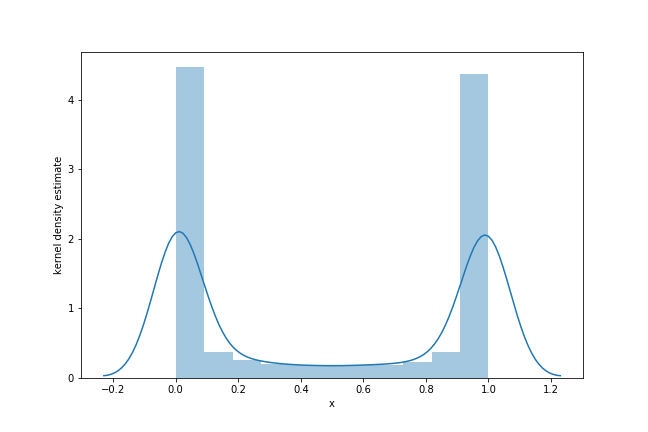
\includegraphics[width=\linewidth]{images/beta_example.png}
 \caption{Kernel Density Plot of the Beta($0.1$, $0.1$) Distribution}
 \label{fig:beta_example}
\end{figure}

More importantly, these distributions cannot be multimodal (with more than $2$ modes), which is the case that is necessary for multiple racial groups and candidates. This is where discretization is most useful. Figure \ref{fig:multimodal_example} is an example of a true multimodal distribution over two variables.

A distribution like this could also be theoretically created with Neural Networks, but that architecture requires tens of thousands, and perhaps millions, of data points to be reliable. The problem of ecological inference is simply too small for those methods.

\begin{figure}[ht]\centering
 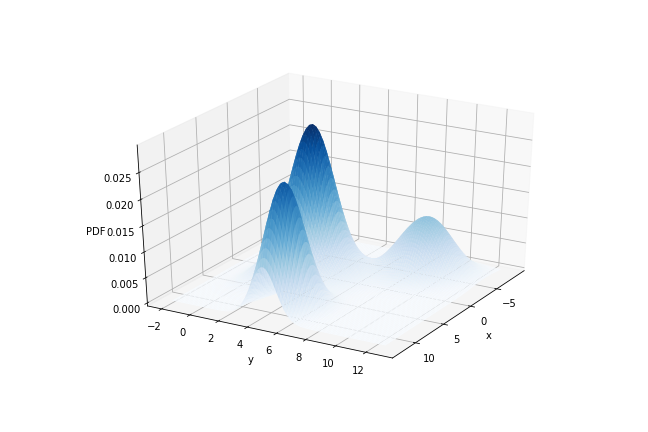
\includegraphics[width=\linewidth]{images/multimodal_example.png}
 \caption{A Bivariate Multimodal Distribution}
 \label{fig:multimodal_example}
\end{figure}

By specifying very little about the space (even less than something like a Beta distribution), then allowing the space to take the shape of the data, more complex, interesting, and possibly accurate distributions can be found. The procedure by which the space takes the shape of the data is Markov chain Monte Carlo.

\subsection{Markov Chain Monte Carlo}

Markov chain Monte Carlo (MCMC) is a class of algorithms that sample from probability distributions that are hard to sample from, typically called \emph{target distributions}.\cite{mcmc_history} With many distributions, like the Normal, Beta, and Exponential mentioned above, obtaining a sample or specifiying those distributions is simple and fast. There exist many packages for Python, R, and other programming languages that generate samples instantly with closed form methods. However, the distribution over the space of hypercubes that could have possibly resulted in the outcome of an election is not well-specified, and differs not only by election, but also by precinct. Hence, applying a well-known distribution requires many approximations and assumptions. In lieu of a well-specified distribution, the Discrete Voter Model uses discretization and MCMC, and in this version specifically, the Metropolis-Hastings algorithm, to find the estimates of the quantities of interest.

The algorithms are iterative, and the idea is that samples converge to the target distribution over time, so the understanding of that target distribution grows with each iteration. In Metropolis-Hastings, each sample is generated from, and only depends on, the prior sample in the process, establishing the Markov relationship. At each step of Metropolis-Hastings, a candidate for the next sample generated according to some proposal rules. That candidate is either accepted or rejected based off of some acceptance probability.

In theory, by the Markov chain central limit theorem, MCMC guarantees convergence and accurate sampling with the correct specifications. Furthermore, the chains are robust to their assumptions, in that they often converge to reliable samples in enough time even when assumptions are broken. Their main disadvantages are that it is difficult to assess convergence for complex distributions and the methods themselves are computationally expensive. However, given the increasing availability of computing power, these methods can be more widely applied.

Hence, these methods are well-suited to the problem of ecological inference, and are implemented in the Discrete Voter Model.

%------------------------------------------------

\newpage
\section{Methods}

All of the methods discussed are implemented in Python, and can be found in the repository noted in the \hyperref[sec:appendix]{appendix}.

The Discrete Voter Model can be divided into $5$ subroutines, each discussed below:

\begin{enumerate}[noitemsep]
  \item \texttt{make\_grid}: create a probabilistic hypercube: an $\mathbf{R}^n$ array of values, $\omega$, that all sum to $1$
  \item \texttt{shift\_weight}: shift weight in a hypercube reversibly
  \item \texttt{expec\_votes}: given a hypercube, a candidate, and a district description, output the expectation of votes that candidate received
  \item \texttt{prob\_votes}: given a hypercube, a candidate, a district description, and the observed vote outcomes, output the probability of seeing that outcome
  \item \texttt{mcmc}: run a Markov Chain Monte Carlo method on a state space of hypercubes
\end{enumerate}

\subsection{\texttt{make\_grid}}

The \texttt{make\_grid} subroutine starts the discretization by initializing an $R^n$ space as a probabilistic hypercube (or grid in the $2$-dimensional case), where $n$ is the number of demographic or racial groups in the electorate.

This hypercube represents the probability distribution of the voting patterns of different demographic groups in a precinct. Each cell in the hypercube corresponds to some collection of $b_i$, the unobserved quantity of interest from King's specification and the necessary quantity for determining racially polarized voting. The cell itself contains the probability of it being the collection that produced the observed outcomes.

The following four subroutines support and implement the MCMC section of the Discrete Voter Model.

\subsection{\texttt{shift\_weight}}

The \texttt{shift\_weight} subroutine implements the proposal step of the MCMC method. It reversibly shifts the weight of the hypercube to create another hypercube. \textit{Reversibility} refers to an assumption of MCMC that guarantees convergence. A Markov chain is said to be reversible if there is a probability distribution, $\pi$, over the states such that:

$$\pi_i \text{Pr}(X_{n+1} = j | X_n = i) = \pi_j \text{Pr}(X_{n+1} = i | X_n = j)$$

for all iterations $n$ and all states $i$ and $j$. This is also called the \textit{detailed balance} condition.

\texttt{shift\_weight} allows for $5$ types of shifting:

\begin{enumerate}[noitemsep]
  \item \texttt{uniform}: add a uniform random hypercube to the hypercube
  \item \texttt{single\_uniform}: add a single uniform random variable to each cell in the hypercube
  \item \texttt{shuffle}: shuffle the hypercube randomly
  \item \texttt{right}: shift weight in the hypercube to the right
  \item \texttt{left}: shift weight in the hypercube to the left
\end{enumerate}

Each of the above types of shifting is reversible, with the \texttt{uniform} as the default method. At each step of the chain, the algorithm uses this subroutine to propose a new hypercube.

\subsection{\texttt{expec\_votes}}

This is the first of two subroutines that score a candidate hypercube in every step of the Markov chain.

\texttt{expec\_votes} calculates the expectation of votes for a given candidate from some probabilistic hypercube.

The subroutine iterates over every cell in the hypercube and finds the expectation of votes that it dictates.

The notation is as follows:

\begin{itemize}[noitemsep]
  \item $i = 0, 1, \dots, n$ represents cells in the hypercube
  \item $p_i$ represents the probability of being in cell $i$
  \item $j = 0, 1, \dots, r$ represents demographic groups
  \item $q_j$ represents the probability of demographic group $j$ to vote for the given candidate
  \item $m_j$ represents the population of demographic group $j$ in the district
\end{itemize}

The expectation of a hypercube is thus given by Equation \ref{eq:expec_votes}.

\begin{equation}
 \sum_{i = 0}^n p_i \left(\sum_{j = 0}^r q_j \cdot m_j\right)
 \label{eq:expec_votes}
\end{equation}

This expectation is then compared to the observed outcome of votes, with the $L1$-norm (absolute value). The lower the norm, the better the hypercube, and the more likely it will be accepted in the Markov chain.

\subsection{\texttt{prob\_votes}}

The is the second of two subroutines that score a candidate hypercube in every step of the Markov chain.

\texttt{prob\_votes} calculates the probability that a given hypercube produced the observed election outcome.

With the same notation as \texttt{expec\_votes}, and additionally:

\begin{itemize}[noitemsep]
  \item $a_j$ represents the number of people in demographic group $j$ that voted for a candidate
  \item $d$ represents the observed number of votes cast for the given candidate
\end{itemize}

\begin{equation}
 \sum_{\forall a_j \text{ s.t. } \sum_{\forall j \in [0, r]} a_j = d} \left(\prod_{j = 0}^r q_j^{a_j} \cdot (1 - q_j)^{m_j - a_j}\right) \cdot \frac{d!}{\prod_{a_j}a_j!}
 \label{eq:prob_votes}
\end{equation}

In essence, Equation \ref{eq:prob_votes} uses the Binomial distribution to calculate the probability of members of different demographic groups voting together in a way to produce the desired outcome. This is extensible to any number of demographic groups and can be repeated for any number of candidates.

A crucial step in this process is generating all possible partitions of the observed electoral outcome into the demographic groups. For example, if $10$ people voted for a candidate, if there are three demographic groups, possible partitions include:

\begin{itemize}
  \item $4$ people from group $1$, $3$ people from group $2$, and $3$ people from group $3$ voted for the candidate
  \item $2$ people from group $1$, $0$ people from group $2$, and $8$ people from group $3$ voted for the candidate
  \item $4$ people from group $1$, $4$ people from group $2$, and $2$ people from group $3$ voted for the candidate
\end{itemize}

The code for this partitioning process can be found in the appendix, as Listing \ref{lst:integer_partition}.

The probability of some candidate hypercube producing the electoral outcome given by that expression is then compared to the probability that the current hypercube produced the outcome, and the candidate is accepted if the probability is higher, or with some acceptance probability if lower.

\subsection{\texttt{mcmc}}

The final subroutine, \texttt{mcmc}, runs the Markov chain Monte Carlo method with the Metropolis-Hastings algorithm, employing either \texttt{expec\_votes} or \texttt{prob\_votes} to score candidates.

The algorithm is as follows:

\begin{enumerate}[noitemsep]
  \item initialize some hypercube with \texttt{make\_grid}
  \item iterate some number of times. at each iteration:
  \begin{enumerate}
    \item generate a candidate hypercube \\ with \texttt{shift\_weight}
    \item score that candidate with \\ \texttt{expec\_votes} or \texttt{prob\_votes}
    \item accept (assign it as the current hypercube and record the score) or reject that candidate based on the scores in the previous step
    \item if the score is better than all scores seen up until this point, save the score and the hypercube
  \end{enumerate}
  \item output all hypercubes explored, and identify the best scoring one
\end{enumerate}

The subroutine returns a collection of the best scoring hypercube, the highest score it received, and a list of all the hypercubes explored and their scores.

\subsection{Evaluation}

All of the methods for inferring racially polarized voting noted above, including ecological regression, homoegenous precincts, and King's EI, are necessarily imperfect -- as is the Discrete Voter Model. The extent of that imperfection, however, can be evaluated and compared.

King's EI and the Discrete Voter Model are evaluated in this paper in two ways: accuracy and runtime. Both models are run on generated election data with different demographic distributions. The evaluation is only possible because with this generated election data, the ground truth, that is: the true demographic voting patterns, is known. That ground truth is fixed as an input in the \texttt{generate\_random\_election} subroutine, whose Python implementation can be found in Listing \ref{lst:election}.

The accuracy of the model is determined by how close the model's result is to the ground truth. The runtime of the model is how long it took the model to reach that result. Both are critically important to the model's use in practice.

DVM's runtime and accuracy are scored in comparison to King's EI for $2 \times 2$ examples, and demonstrations of its use on $R \times C$ examples are given in the \hyperref[sec:results]{Results} section.

%------------------------------------------------

\newpage
\section{Results}
\label{sec:results}

\subsection{Experiment Specification}

\bm{$2 \times 2$} \textbf{Case}

For the $2$ demographic group case, $5$ random elections were generated for each of the demographic distributions of the precicnt in Table \ref{table:demo_dist} for precincts of size $100$. Each of these distributions is labeled $d_i \forall i \in [1, 3]$ (without loss of generality) for reference in Table \ref{table:results}.

The true demographic voting patterns for candidates $a$ and $b$ in Table \ref{table:voting}. Each of these voting patterns is labeled $v_i \forall i \in [1, 2]$ (without loss of generality) for reference in Table \ref{table:results}.

\begin{table}[ht]
 \centering
 \caption{Demographic Distributions Tested in the $2 \times 2$ Case}
 \label{table:demo_dist}
 \begin{tabular}{|c|c|c|}
   \hline
   Label & Group $1$ ($\%$) & Group $2$ ($\%$) \\
   \hline
   $d_1$ & $50$ & $50$ \\
   $d_2$ & $25$ & $75$ \\
   $d_3$ & $10$ & $90$ \\
  \hline
 \end{tabular}
\end{table}

\begin{table}[ht]
 \centering
 \caption{Demographic Voting Patterns Tested in the $2 \times 2$ Case}
 \label{table:voting}
 \begin{tabular}{|c|c|c|c|}
   \hline
   Label & Group & Cand. $a$ ($\%$) & Cand. $b$ ($\%$) \\
   \hline
   \multirow{2}{*}{$v_1$} & $1$ & $50$ & $50$ \\
   & $2$ & $30$ & $70$ \\
   \hline
   \multirow{2}{*}{$v_2$} & $1$ & $25$ & $75$ \\
   & $2$ & $20$ & $80$ \\
  \hline
 \end{tabular}
\end{table}

\bm{$3 \times 2$} \textbf{Case}

For the $3$ demographic group cases, $5$ random elections were generated for each of the demographic distributions of the precinct in Table \ref{table:demo_dist_3} precincts of size $100$. Each of these distributions is labeled $d_i \forall i \in [4, 6]$ (without loss of generality) for reference in Table \ref{table:results}.

The true demographic voting patterns for candidates $a$ and $b$ in Table \ref{table:voting_3}. Each of these voting patterns is labeled $v_i \forall i \in [3, 4]$ (without loss of generality) for reference in Table \ref{table:results}.

\begin{table}[ht]
 \centering
 \caption{Demographic Distributions Tested in the $3 \times 2$ Case}
 \label{table:demo_dist_3}
 \begin{tabular}{|c|c|c|c|}
   \hline
   Label & Group $1$ ($\%$) & Group $2$ ($\%$) & Group $3$ ($\%$) \\
   \hline
   $d_4$ & $50$ & $50$ & $0$ \\
   $d_5$ & $25$ & $25$ & $50$ \\
   $d_6$ & $33$ & $33$ & $34$ \\
  \hline
 \end{tabular}
\end{table}

\begin{table}[ht]
 \centering
 \caption{Demographic Voting Patterns Tested in the $3 \times 2$ Case}
 \label{table:voting_3}
 \begin{tabular}{|c|c|c|c|}
   \hline
   Label & Group & Cand. $a$ ($\%$) & Cand. $b$ ($\%$) \\
   \hline
   \multirow{3}{*}{$v_3$} & $1$ & $20$ & $80$ \\
   & $2$ & $80$ & $20$ \\
   & $3$ & $40$ & $60$ \\
   \hline
   \multirow{3}{*}{$v_4$} & $1$ & $30$ & $70$ \\
   & $2$ & $40$ & $60$ \\
   & $3$ & $50$ & $50$ \\
  \hline
 \end{tabular}
\end{table}

\subsection{Accuracy and Runtime}

Accuracy is reported as the mean squared error (MSE) between the models' outputted demographic voting distribution and the true demographic voting distribution, averaged over all trials. The lower the MSE, the more accurate the model. The runtime is in seconds. The lower the runtime, the faster the model.

Table \ref{table:results} summarizes the results of running DVM and King's EI on all of the experiments, for a total of $12$ experiments replicated $5$ times each, in Python 3.7.4 on a 2018 MacBook Pro with a 2.3 GHz Quad-Core Intel Core i5 processor, 16 GB of 2133 MHz LPDDR3 RAM, and a Intel Iris Plus Graphics 655 1536 MB graphics card. All numbers are given with $3$ significant figures of precision. The DVM's MCMC was configured with $200$ steps, and the hypercubes had a granularity of $10$.

\begin{table}[ht]
 \centering
 \caption{Accuracy and Runtime of the Discrete Voter Model (DVM) and King's EI (KEI)}
 \label{table:results}
 \begin{tabular}{|c|c|c|c|c|}
   \hline
   & \multicolumn{2}{|c|}{DVM} & \multicolumn{2}{|c|}{KEI} \\
   \hline
   Label & MSE & Runtime (s) & MSE & Runtime (s) \\
   \hline
   $d_1 \times v_1$ & $0.0825$ & $3.08$ & $0.0253$ & $13.9$ \\
   $d_1 \times v_2$ & $0.0893$ & $3.04$ & $0.0589$ & $14.0$ \\
   \hline
   $d_2 \times v_1$ & $0.153$ & $4.05$ & $0.0665$ & $16.9$ \\
   $d_2 \times v_2$ & $0.194$ & $2.89$ & $0.0604$ & $11.5$ \\
   \hline
   $d_3 \times v_1$ & $0.107$ & $2.74$ & $0.0134$ & $9.77$ \\
   $d_3 \times v_2$ & $0.103$ & $2.72$ & $0.0620$ & $9.55$ \\
   \hline
   $d_4 \times v_3$ & $0.0692$ & $1500$ & - & - \\
   $d_4 \times v_4$ & $0.0825$ & $1470$ & - & - \\
   \hline
   $d_5 \times v_3$ & $0.236$ & $1570$ & - & - \\
   $d_5 \times v_4$ & $0.156$ & $1530$ & - & - \\
   \hline
   $d_6 \times v_3$ & $0.149$ & $1530$ & - & - \\
   $d_6 \times v_4$ & $0.125$ & $1500$ & - & - \\
  \hline
 \end{tabular}
\end{table}

In addition to the presentation of the numeric evaluation, a presentation of select visualizations of the models produced by the Discrete Voter Model show its expressive power.

Figure \ref{fig:2d_viz} shows the distribution of probability over the $2$D hypercube for a model in the $2 \times 2$ case. The figure is $3$-dimensional, with the third dimension being the probability of being in one of the cells of the hypercube. This is multinomial and much more expressive of possible outcomes.

\begin{figure}[ht]\centering
 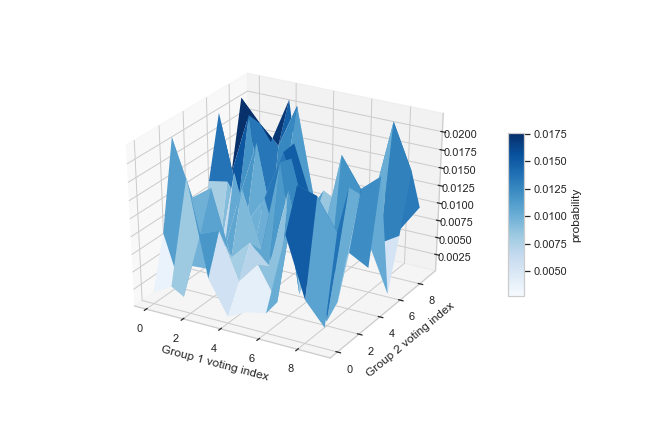
\includegraphics[width=\linewidth]{images/2d_viz.png}
 \caption{Distribution of Probability over the 2D Hypercube for a Model in the $2 \times 2$ Case}
 \label{fig:2d_viz}
\end{figure}

Figure \ref{fig:3d_viz} shows the distribution of probability over the $2$D hypercube for a model in the $3 \times 2$ case. Since there are $3$ dimensions for demographic groups, Figure \ref{fig:3d_viz} presents the fourth dimension, probability, as directed arrows across a cross section of the dimensions. The colors of these arrows give the corresponding probability.

\begin{figure}[ht]\centering
 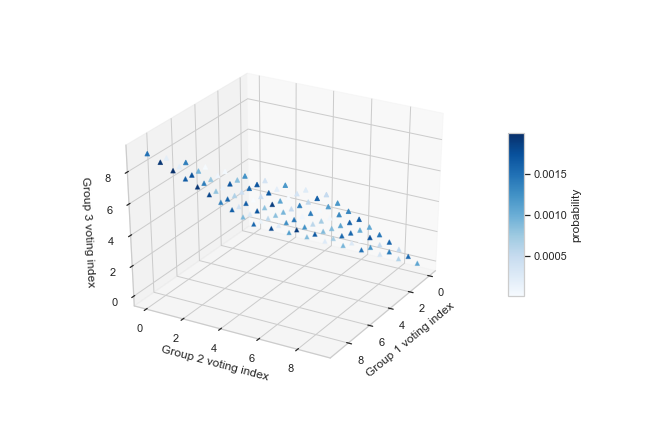
\includegraphics[width=\linewidth]{images/3d_viz.png}
 \caption{Distribution of Probability over the 3D Hypercube for a Model in the $3 \times 2$ Case}
 \label{fig:3d_viz}
\end{figure}


%------------------------------------------------
\newpage
\section{Discussion and Conclusion}
\label{sec:conclusion}

The results presented in Table \ref{table:results} show three primary trends:

\begin{enumerate}[noitemsep]
  \item the Discrete Voter Model performs nearly as well as, but a little worse than, King's Ecological Inference in the $2 \times 2$ case (two demographic groups and two candidates)
  \item the Discrete Voter Model is remarkably faster than King's Ecological Inference in the $2 \times 2$ case (two demographic groups and two candidates)
  \item unlike King's EI, the Discrete Voter Model can produce reliable results for the $3 \times 2$ case (three demographic groups and two candidates)
\end{enumerate}

The Discrete Voter Model was limited to $200$ steps, with a hypercube granularity of $10$ (that is, each dimension of the cube went from $0$ to $9$). Further testing corroborates the theory that, generally, with more iterations, Markov chain Monte Carlo converges to the true distribution. Hence, allowing DVM to run longer may increase the accuracy of the model, at the expense of runtime.

With that said, DVM was able to use those $200$ steps to perform comparably to King's EI in the $2 \times 2$ cases. This also corresponded to a lower runtime than King's EI in all cases, which is a testament to improvements in computing power and algorithms.

DVM was also able to do what King's EI cannot in any amount of time: run on the larger $3 \times 2$ tables. Higher dimensional tables are also possible with DVM, with no changes to the statistical theory or implementation.

If King's EI is taken to be a standard method, as it has been by some courts, DVM's performance on these generated elections show that it is a good contender. Not only does it perform comparably, but:

\begin{itemize}
  \item it is inherently extensible and can be tuned. Generally, at the expense of time:
  \begin{itemize}
    \item one can increase the number of iterations to get closer to the true distribution
    \item one can increase the size of the hypercube to get more granular estimates for the racial voting patterns
  \end{itemize}
  \item it can produce visualizations of more complex voting pattern distributions
\end{itemize}

The Discrete Voter Model leverages the power of discretization and Markov chain Monte Carlo to provide more expressive models within a more malleable and sound structure. Its flexibility has been shown on generated election data, and improvements continue to be made to its speed.

As Jim Greiner said: "Racial bloc voting, often a hotly contested issue in an "ordinary" redistricting dispute, may now become even more so, and as a result, using the best methodology is more critical."\cite{greiner} The Discrete Voter Model, as presented here and in future iterations, is a direct response to the need for more flexible and robust methods in the redistricting and voting rights space.

%------------------------------------------------
\phantomsection
\section*{Acknowledgments}
\addcontentsline{toc}{section}{Acknowledgments}

I would like to express my deep gratitude to Professor Latanya Sweeney, Jinyan Zang, and the students of the Fall 2019 iteration of GOV93B at Harvard University. They provided me with patient guidance, enthusiastic encouragement and useful critiques of the scope and design of this research work. In addition, I would like to thank Professor Moon Duchin of Tufts University for her guidance of this research and my overall thesis work.


%	REFERENCE LIST
\phantomsection
\bibliographystyle{unsrt}
\bibliography{references}

% APPENDIX

\onecolumn
\phantomsection
\section*{Appendix}
\label{sec:appendix}
\addcontentsline{toc}{section}{Appendix}
\subsection*{Code Snippets}

The full set of code for this research and method can be found \href{https://github.com/hangulu/thesis}{here}. To completely reproduce these experiments, run \texttt{methods.ipynb} in full. The following are notable code snippets mentioned in the body of the article.

\insertcode{"code/ei.py"}{Python Implementation of King's Ecological Inference}{lst:ei_code}

\insertcode{"code/partition.py"}{Integer Partitioning}{lst:integer_partition}

\insertcode{"code/election.py"}{Generate a Random Election}{lst:election}

\insertcode{"code/eval.py"}{Evaluate and Compare DVM and King's EI}{lst:eval}


\end{document}
